A \textbf{cryptographic module} is a set of hardware, software, firmware, or some combination thereof that implements cryptographic computations within a contiguous perimeter defining the physical or logical boundaries of the module \cite{nist_security_2019}. \textbf{Software-based cryptographic modules} correspond to any kind of software implementing cryptographic computations for general-purpose hardware, while \textbf{hardware-based cryptographic modules} correspond to dedicated hardware implementing cryptographic computations through ad-hoc circuits \cite{csa_key_2020}. Below, we briefly present popular hardware-based cryptographic modules (\Cref{table:hardware_comparison}) and compare hardware- and software-based cryptographic modules (\Cref{sec:cryptographic_modules:software}).


\subsection{Hardware Security Modules}\label{sec:cryptographic_modules:hsm}

A \gls{hsm} (\Cref{figure:hsm}) is a physical device --- either pluggable or standalone --- specifically designed to provide a complete solution for algorithm execution and secure key management (\Cref{sec:key_management}). \glspl{hsm} implement a dedicated operating system and allow for defining \gls{ac} policies 
%TODO (\Cref{future_sec:access_control})
to mediate requests --- sent on a secure channel --- toward their \glspl{api}. \glspl{hsm} are thoroughly tested and built with specialized hardware (usually certified by third-party regulators --- see \Cref{sec:standards_and_certifications}) offering protection against physical, chemical, or mechanical tampering. Furthermore, \glspl{hsm} are usually equipped with sensors to detect attacks (such as drilling, breaking open, or applying acid to the casing) and trigger proper countermeasures (e.g., automatic erase of all keys stored within the \gls{hsm}) --- this property is often called \textbf{tamper responsiveness}.

\curiosityBlock{How much does an \gls{hsm} cost?}{\glspl{hsm} are expensive hardware costing on average between 10.000€ and 20.000€ (cheaper alternatives are of course available but may present security and performance trade-offs). For this reason, \glspl{hsm} are usually used at the server side only as the first building block for implementing \glspl{kms}.}

\begin{figure}[t!]
	\begin{center}
		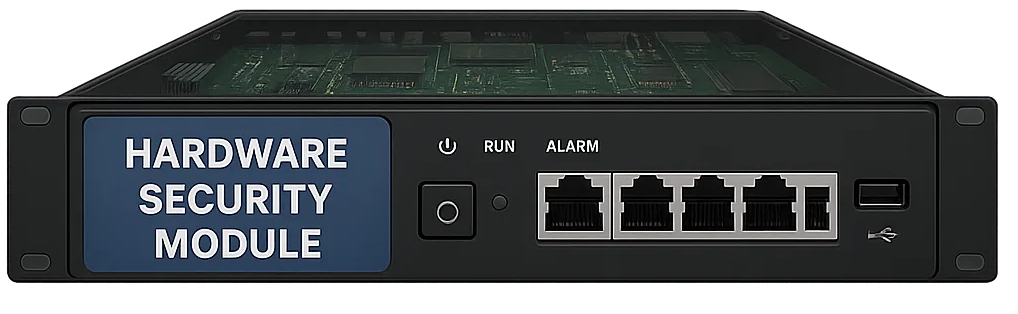
\includegraphics[width=0.8\linewidth]{resources/img/hsm.png}
		\caption{A generic \gls{hsm} where the top lid was made transparent only for showing the internal circuitry; of course, the case of an \gls{hsm} is typically made entirely with metal (image generated with OpenAI's Sora --- \url{https://sora.chatgpt.com/}).}
		\label{figure:hsm}
	\end{center}
\end{figure}

\glspl{hsm} provide \glspl{trng}
%TODO (\Cref{future_sec:randomness}) 
based on physical processes (e.g., atomic decay or atmospheric noise). Besides, \glspl{hsm} can execute (usually but not necessarily predefined) algorithms securely through dedicated cryptoprocessors, and some new \glspl{hsm} may even run arbitrary code. Finally, \glspl{hsm} allows exporting keys, usually previously encrypted with a key derived from a \gls{pbkdf} (\Cref{sec:key_management:lifecycle:pre}); in this regard, it is important to note that, while preventing a \gls{spof}, exporting a key from a \gls{hsm} degrades the security of that key (as an attacker may then be able to steal it and perform an offline guessing attack --- see \Cref{sec:cryptographic_security_overview:attacks}). 


\subsection{Secure Elements}\label{sec:cryptographic_modules:se}

\begin{figure}[t!]
	\begin{center}
		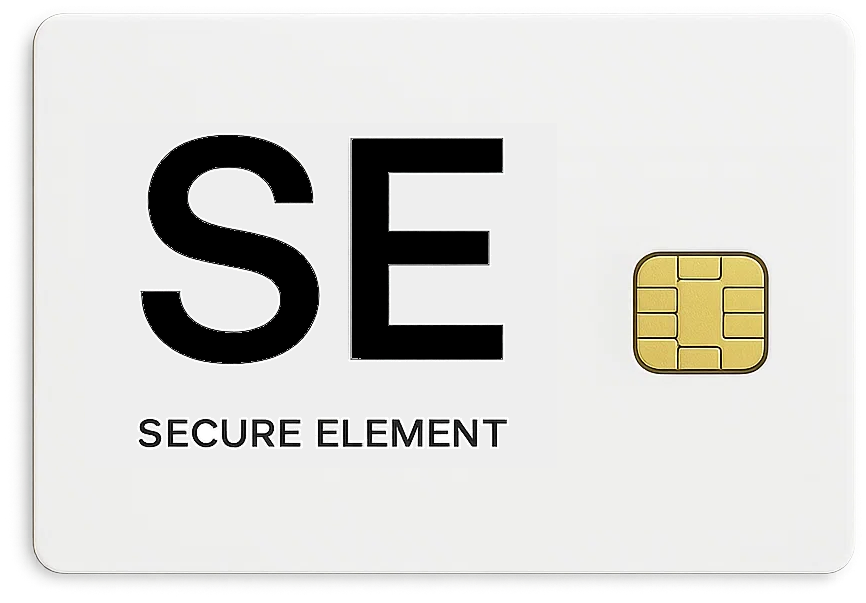
\includegraphics[width=0.4\linewidth]{resources/img/se.png}
		\caption{A generic \gls{se} (image generated with OpenAI's Sora --- \url{https://sora.chatgpt.com/}). Note that \glspl{se} come in a wide variety of fashions.}
		\label{figure:se}
	\end{center}
\end{figure}

A \gls{se} (\Cref{figure:se}) is a chip --- either discrete, pluggable, or integrated --- capable of storing secrets and executing preloaded algorithms packaged as (usually Java) applets. \glspl{se} almost always has limited storage capacity and processing speed --- often because \glspl{se} receive power by induction. Besides, \glspl{se} are typically tamper-resistant and provide access restriction for trusted applications only.

\remarkBlock{Formats for \glspl{se}}{\glspl{se} have a wide range of implementations such as SIM cards, EMV chips, smart microSD, smart cards, cryptographic tokens, hardware digital wallets, and embedded circuits. \glspl{se} are either portable or embedded in mobile devices.}


\subsection{Trusted Platform Modules}\label{sec:cryptographic_modules:tpm}

\begin{figure}[t!]
	\begin{center}
		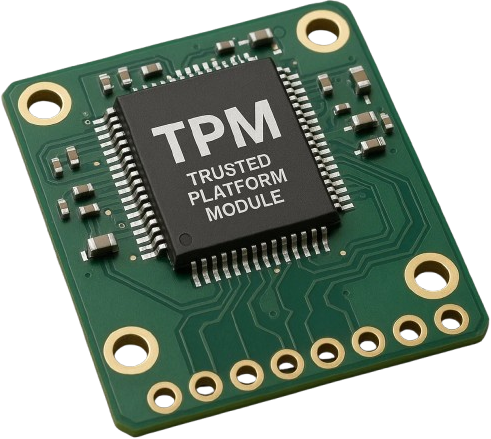
\includegraphics[width=0.4\linewidth]{resources/img/tpm.png}
		\caption{A generic \gls{tpm} (image generated with OpenAI's Sora --- \url{https://sora.chatgpt.com/}).}
		\label{figure:tpm}
	\end{center}
\end{figure}

A \gls{tpm} (\Cref{figure:tpm}) is a chip either plugged or soldered into the motherboard of devices capable of storing secrets (usually keys, certificates, and passwords) and executing predefined algorithms through dedicated cryptoprocessors. \glspl{tpm} are mainly used as \textbf{hardware roots of trust}\footnote{A hardware root of trust is a dedicated, inherently trusted hardware component --- most often, a tamper-resistant cryptographic module --- containing private or secret cryptographic material that serves as a foundational security anchor. Typically, such cryptographic material is endorsed by a \gls{pki} (\Cref{sec:binding_keys_to_parties:pki}).} --- \glspl{tpm} do not have general computational capacity --- and are typically equipped with:
\begin{itemize}
	\item an \textbf{endorsement key} created during the manufacturing process. The endorsement key cannot be exported and can be used for authenticating the \gls{tpm} --- and, consequently, the device where the \gls{tpm} is installed;
	\item a \textbf{storage root key}, either built-in or (more often) derived from the endorsement key and a password specified by the owner of the device where the \gls{tpm} is installed. The storage root key cannot be exported and is typically used as \gls{kek} (\Cref{sec:cryptography_basics:keys});
	\item an \textbf{attestation identity key} used to protect the \gls{tpm} against tampering attempts on its firmware through \glspl{mac} (\Cref{sec:symmetric_cryptography:mac}).
\end{itemize}

\glspl{tpm} are usually found in laptops and desktop computers, as their adoption in mobile devices has been hindered by computational, energy, and monetary constraints.

\curiosityBlock{The history of the \gls{tpm}}{The first version of the \gls{tpm} dates back to 2003, while the latest \gls{tpm} version (2.0) dates back to 2012 --- the organization standardizing \glspl{tpm} is the \gls{tcg}.\footnote{Trusted Platform Module (TPM) | Trusted Computing Group (TPM) (\url{https://trustedcomputinggroup.org/work-groups/trusted-platform-module/})}}


\subsection{Trusted Execution Environments}\label{sec:cryptographic_modules:tee}

\begin{figure}[t!]
	\begin{center}
		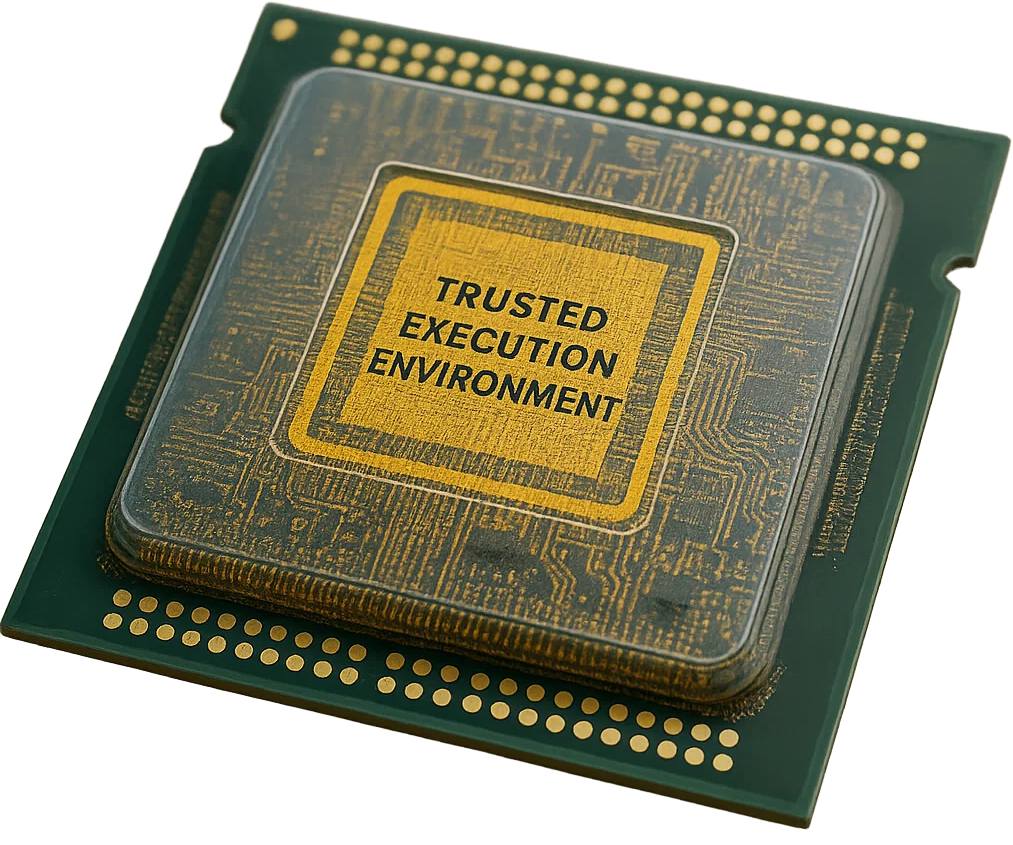
\includegraphics[width=0.4\linewidth]{resources/img/tee.png}
		\caption{A generic \gls{tee} (image generated with OpenAI's Sora --- \url{https://sora.chatgpt.com/}).}
		\label{figure:tee}
	\end{center}
\end{figure}

A \gls{tee} (\Cref{figure:tee}) is a dedicated area of the main processor of a device (laptops, desktop computers, mobile, and even \gls{iot} devices) --- hence, separated from the operating system --- allowing to run applications with access to the resources of the device itself securely. At a high level, \glspl{tee} can easily run arbitrary code and are often used for digital wallets, secure booting (although \glspl{tpm} are more apt at that), mobile payments, and (especially) confidential computing\footnote{Confidential Computing Consortium (\url{https://confidentialcomputing.io/})} \cite{munoz_survey_2023}. 

\readBlock{More information on Confidential Computing}{The article ``Toward Confidential Cloud Computing'' \cite{russinovich_toward_2021} is an excellent introductory resource on confidential computing in the cloud, starting from why it may be necessary, what are the technologies involved, and what applications it may have.}

GlobalPlatform\footnote{GlobalPlatform: Securing the Digital Future (\url{https://globalplatform.org/})} is the main (non-profit) organization defining \glspl{tee}' architectures and supporting the standardization of \glspl{tee}'s technical specifications and capabilities. Hence, although \glspl{tee} may be implemented with fundamentally different technologies --- and their level of security may vary accordingly --- basic features inherent to any (or at least the vast majority of) \glspl{tee} are \cite{sabt_trusted_2015}:

\begin{itemize}
	\item \textbf{remote attestation}, which allows for verifying the integrity (hence, the trustworthiness) of the \gls{tee} and its contents; one possible implementation involves generating a report containing measurements of the \gls{tee}'s status (e.g., deployed software, firmware) using cryptographic hash functions: the report is signed with a dedicated private key and sent to an \textbf{attestation authority} --- a trusted third party that usually coincides with the manufacturer of the \gls{tee} --- which verifies the signature of the report and compares the measurements contained therein against expected values. A standardized architecture for remote attestation called \gls{rats} was proposed by the \gls{ietf} in \cite{rfc9334};
	\item \textbf{isolated execution}, which protects data and software running within the \gls{tee}. More precisely, \glspl{tee} usually preserve the confidentiality and the integrity of data contained therein, and the integrity (but not the confidentiality) of the software executed therein --- still, note that it is possible to preserve the confidentiality of sensitive code by, e.g., treating it as data consequently executed by a (public) interpreter or by decrypting (encrypted) sensitive code within the \gls{tee} (e.g., see \cite{quarta_tarnhelm_2021}). Importantly, isolated execution may occur either at the \textbf{\gls{vm} level} or at the \textbf{application level} (the latter is also referred to as \textit{process level}):\footnote{Current Trusted Execution Environment landscape - Red Hat Emerging Technologies (\url{https://next.redhat.com/2019/12/02/current-trusted-execution-environment-landscape/})}
	\begin{itemize}
		\item \textit{application-level isolated execution}: protection at the application level separates the execution of software (e.g., of an application) between two \textbf{worlds} or \textit{realms}: the secure world (inside the \gls{tee}) and the normal world (the main processor). The (portion of the) software running inside the secure world is usually referred to as \textbf{trusted application} or \textit{trustlet} (inspired by the term ``applet''), whereas the software running inside the normal world is referred to as \textbf{untrusted application}. The combination of the trusted application together with the (computational resources and security perimeter) of the secure world is often called enclave.\footnote{enclave - Glossary | CSRC (\url{https://csrc.nist.gov/glossary/term/enclave})} Untrusted applications interface with the operating system and can interact with trusted applications only through well-defined interfaces. Trusted applications are generally limited in size, constituting a small \gls{tcb} (\Cref{sec:programming_languages_and_software:trusted_computing_base}). Note that even users cannot access data and code of their own trusted applications --- that is, users interact with the \gls{tee} as a black box. Finally, the development of software intended for application-level isolated execution typically relies on \gls{tee}-specific \gls{sdk} and \glspl{api};
		\item \textit{\gls{vm}-level isolated execution}: protection at the \gls{vm} level targets software packaged as \glspl{vm} and protects them from the underlying hypervisor, providing isolation between the \glspl{vm} and the operating system --- and also among the \glspl{vm} themselves. Consequently, the entire \gls{vm} constitutes a (large) \gls{tcb}. Note that users have a certain degree of transparency and visibility on the (data and code running within) their own \glspl{vm} --- for instance, the owner of a \gls{vm} has full read and write access over the \gls{vm}, which may be too coarse in many cases. \cite{russinovich_toward_2021}. Finally, the development of software intended for \gls{vm}-level isolated execution does not have any particular requirements and does not need to interact with any \gls{tee}'s specific \glspl{api};
		\remarkBlock{Isolated execution for containers}{Containers are small standalone executable packages that contain software --- usually, a single program --- along with its dependencies. Containers are widely popular nowadays and, roughly speaking, can be seen as a middle way between simple applications and \glspl{vm}. Hence, containers may ideally be executed with either application-level or (most often) \gls{vm}-level isolated execution.}
	\end{itemize} 
	\item \textbf{secure channels}, which allows for establishing local (e.g., I/O) and remote communication channels for data transmission protected against external attacks (e.g., key-logging, replay, eavesdropping, tampering).
\end{itemize}

Intuitively, some \gls{tee} implementations --- see \Cref{sec:cryptographic_modules:tee:implementations} --- may offer further features (e.g., data sealing, resistance to side-channel attacks, obliviousness).

\remarkBlock{On the practicality of developing software for \glspl{tee}}{Developing software for \glspl{tee}, especially for those offering application-level isolated execution, often leads to lock in to specific \glspl{sdk}, technologies, or features, and compatibility issues among software versions. Still, projects offering abstractions over \glspl{tee} to simplify development exist, e.g., Open Enclave SDK.\footnote{SDK for developing enclaves (\url{https://github.com/openenclave/openenclave})}}

\subsubsection{Trusted Execution Environment Implementations}\label{sec:cryptographic_modules:tee:implementations}

The authors in \cite{munoz_survey_2023} report a list of \gls{tee} implementations among which we highlight:
\begin{itemize}
	\item \textbf{TrustZone by ARM},\footnote{TrustZone technology for the ARMv8-M architecture Version 2.0 (\url{https://developer.arm.com/documentation/100690/0200/ARM-TrustZone-technology})} a \gls{tee} for ARM processors offering application-level isolated execution especially popular in mobile and \gls{iot} devices;
	\item \textbf{\gls{sgx} by Intel},\footnote{Intel Software Guard Extensions (\url{https://www.intel.com/content/www/us/en/products/docs/accelerator-engines/software-guard-extensions.html})} a \gls{tee} for Intel processors offering application-level isolated execution which has been deprecated in client-side processors in 2022 due to its (too) many vulnerabilities and --- at the time of writing --- is only available in server-side processors;\footnote{Intel SGX deprecated in 11th Gen processors (\url{https://community.intel.com/t5/Intel-Software-Guard-Extensions/ Intel-SGX-deprecated-in-11th-Gen-processors/m-p/1351848})}
	\item \textbf{Sanctum} \cite{sanctum_costan_2016}, a seminal academic prototype open-source \gls{tee} for RISC-V processors offering application-level isolated execution and introduced in 2016 as an alternative to proprietary solutions like Intel \gls{sgx}. Sanctum has seen limited updates or development in recent years\footnote{The MIT Sanctum processor top-level project (\url{https://github.com/ilebedev/sanctum})};
	\item \textbf{\gls{tdx} by Intel}\footnote{Intel Trust Domain Extensions (Intel TDX)(\url{https://www.intel.com/content/www/us/en/developer/tools/trust-domain-extensions/overview.html})} and \textbf{\gls{sev} by AMD},\footnote{AMD Secure Encrypted Virtualization (SEV) | AMD (\url{https://www.amd.com/en/developer/sev.html})} two \glspl{tee} for Intel and AMD processors, respectively, offering \gls{vm}-level isolated execution often employed in cloud computing environments such as those of Azure\footnote{Azure Confidential VM options | Microsoft Learn (\url{https://learn.microsoft.com/en-us/azure/confidential-computing/virtual-machine-options})} and Google;\footnote{Confidential VM overview | Google Cloud (\url{https://cloud.google.com/confidential-computing/confidential-vm/docs/confidential-vm-overview})}
	\item \textbf{Keystone} \cite{lee_keystone_2020},\footnote{Keystone Enclave (QEMU + HiFive Unleashed) (\url{https://github.com/keystone-enclave/keystone})} an open-source \gls{tee} for RISC-V processors introduced in 2020 inspired from Sanctum;
	\item \textbf{Sancus} \cite{sancus_noorman_2013},\footnote{Minimal OpenMSP430 hardware extensions for isolation and attestation (\url{https://github.com/sancus-tee/sancus-core})} an open-source \gls{tee} comprising OpenMSP430 hardware extensions for \gls{iot} devices.
\end{itemize}

\gls{tee} implementations may have several re-configurations, extensions, or software abstractions known under different names. Hence, it is recommended to always investigate whether a supposedly new \gls{tee} implementation is actually directly built upon on an already existing \gls{tee} implementation (e.g., OP-TEE\footnote{About OP-TEE — OP-TEE documentation (\url{https://optee.readthedocs.io/en/latest/general/about.html})} is a popular software \gls{tee} that runs on ARM TrustZone).


\subsection{Physical Unclonable Functions}\label{sec:cryptographic_modules:puf}

\begin{figure}[t!]
	\begin{center}
		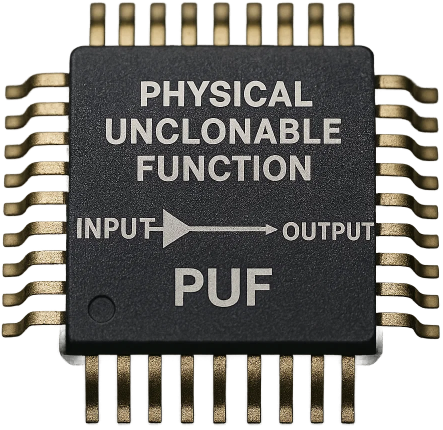
\includegraphics[width=0.4\linewidth]{resources/img/puf.png}
		\caption{A generic \gls{puf} (image generated with OpenAI's Sora --- \url{https://sora.chatgpt.com/}).}
		\label{figure:puf}
	\end{center}
\end{figure}

A \gls{puf} (\Cref{figure:puf}) is a physical circuit that operates based on a challenge-response mechanism, that is, given an input (called \textbf{challenge}), a \gls{puf} returns a physically defined --- and unpredictable a-priori --- \textit{digital fingerprint} output (called \textbf{response}). The challenge-response pairs are unique to each \gls{puf}; in other words, the same challenge produces the same response, while different challenges produce different responses. \glspl{puf} are based on unique physical variations occurring naturally during semiconductor manufacturing; this property means that \glspl{puf} are easy to manufacture but practically impossible to duplicate. \glspl{puf} allow for generating and storing keys --- in the sense that \glspl{puf}, given the same challenge, can re-generate the same key. However, it is not possible to import cryptographic keys into \glspl{puf}.

\begin{table}[!b]
	\centering
	\small
	\setlength{\tabcolsep}{3pt}
	\def\arraystretch{1.075}
	\rowcolors{0}{white}{cloud}
	\caption{Properties of Hardware-based Cryptographic Modules: a full, half, and empty circle (i.e., $\fullcirc$, $\halfcirc$, $\emptycirc$) mean that the corresponding property is supported by the majority of the implementations, some of the implementations, or none of the implementations of the relative hardware-based cryptographic module, respectively. We define as \textbf{Portable} the property of a hardware-based cryptographic module of being easily removable, carried, and used in multiple devices, whereas \textbf{Key Usage} means that cryptographic computations (e.g., encryption) take place entirely within the module}
	\newcolumntype{Y}{>{\centering\arraybackslash}X}
	\begin{tabularx}{\textwidth}{l|YYYYY}
		
		\toprule
		
		\multicolumn{1}{c|}{\textbf{Property}} &
		\multicolumn{1}{c}{\textbf{\gls{hsm}}} &
		\multicolumn{1}{c}{\textbf{\gls{se}}}  &
		\multicolumn{1}{c}{\textbf{\gls{tpm}}} &
		\multicolumn{1}{c}{\textbf{\gls{tee}}} &
		\multicolumn{1}{c}{\textbf{\gls{puf}}} \\
		
		\hline
		
		Tamper Responsive		& \fullcirc 	& \emptycirc 	& \emptycirc 	& \emptycirc 	& \emptycirc	\\
		Portable 				& \fullcirc 	& \halfcirc 	& \emptycirc 	& \emptycirc 	& \emptycirc 	\\
		Key Generation 			& \fullcirc 	& \fullcirc 	& \fullcirc 	& \fullcirc 	& \fullcirc 	\\
		Key Storage 			& \fullcirc 	& \fullcirc 	& \fullcirc 	& \fullcirc 	& \halfcirc		\\
		Key Usage				& \fullcirc 	& \fullcirc 	& \fullcirc 	& \fullcirc 	& \emptycirc 	\\
		Key Export				& \fullcirc 	& \emptycirc 	& \fullcirc 	& \fullcirc 	& \emptycirc 	\\
		Dedicated Processors	& \fullcirc 	& \emptycirc 	& \fullcirc 	& \fullcirc 	& \emptycirc 	\\
		Run Arbitrary Code		& \halfcirc 	& \emptycirc 	& \emptycirc 	& \fullcirc 	& \emptycirc 	\\
		
		\bottomrule
		
	\end{tabularx}
	\label{table:hardware_comparison}
\end{table}


\subsection{Hardware- vs. Software-Based Cryptographic Modules}\label{sec:cryptographic_modules:software}

The choice between hardware- and software-based cryptographic modules entirely depends on the underlying scenario (e.g., availability of hardware devices) and its requirements (e.g., usability vs. security). Nevertheless, it is still possible to provide a high-level comparison between the two kinds of cryptographic modules.

\remarkBlock{Cryptographic modules security standards}{There exist several standards for categorizing and certifying the protection levels --- in terms of security and reliability --- of both hardware- and software-based cryptographic modules (which are commonly certified with a combination of such standards): please refer to \Cref{sec:standards_and_certifications} for more details.}

First, we note that managing sensitive (cryptographic) data and applications in a dedicated hardware environment provides high(er) performance --- thanks to the use of dedicated cryptoprocessors and circuits --- and, especially, high(er) security. Indeed, according to \gls{nist}'s security levels definition in \cite{nist_security_2019}, \textbf{software-based cryptographic modules can reach up to security level 2}, while \textbf{hardware-based cryptographic modules reach up to security level 4}. Moreover, \glspl{trng} require the use of ad hoc appliances which are seldom available on the hosts running software-based cryptographic modules.
%TODO (\Cref{future_sec:randomness}). 
On the other hand, software-based cryptographic modules are highly portable, do not require (expensive) dedicated hardware, and are easier to develop and update.

As for disadvantages, hardware-based cryptographic modules (e.g., \glspl{puf}) may be a \gls{spof} and, in general, it may be difficult to achieve redundancy of cryptographic material contained in hardware-based cryptographic modules without invalidating their security properties (e.g., as said in \Cref{sec:cryptographic_modules:hsm}, exporting keys from a \gls{hsm} reduced the security of the keys). Hardware-based cryptographic modules are also opaque, meaning that it is usually impossible to inspect or monitor cryptographic computations executed within. Moreover, the intrinsic resilience to external modifications makes hardware-based cryptographic modules difficult to update in case vulnerabilities are found --- which is not infrequent. Finally, it is important to note that, although manufacturers can release patches and fix vulnerabilities, often already existing hardware cannot be updated.

\warningBlock{On the (in)security of hardware-based cryptographic modules}{Hardware-based cryptographic modules are not bullet-proof and have been successfully attacked several times and in very different ways: \glspl{se} are particularly exposed to side-channel attacks (\Cref{sec:security_of_cryptographic_algorithms:attacks}), \glspl{tee} are often subject --- besides to side-channel attacks --- also to software-based and (micro)architectural attacks (see \cite{munoz_survey_2023} for a nice survey), and \glspl{hsm} has been vulnerable to firmware tampering and secret extraction attacks.\footnote{Black Hat USA 2019 | Briefings Schedule (\url{https://www.blackhat.com/us-19/briefings/schedule/\#everybody-be-cool-this-is-a-robbery-16233})} The history of the (in)security of hardware-based cryptographic modules does not mean that they are useless, but rather that their adoption should occur in full awareness of their limits and require a thorough risk assessment.\footnote{risk assessment - Glossary | CSRC (\url{https://csrc.nist.gov/glossary/term/risk_assessment})} Furthermore, note that relying on hardware-based cryptographic modules entails trusting the cryptographic modules' manufacturers. In some applications, e.g., confidential computing, this translates into a trust shift from cloud providers to manufacturers (in other words, you always end up trusting someone else).}
